\section{Combinatorial semantics}

\section{String Diagram Rewrite Theory}\label{sec:combinatorial-semantics}

In this section,  we recall the fundamental definitions and results of string diagram rewrite theory for symmetric monoidal categories,  building to the recapitulation of the correspondence between string diagram rewriting and an appropriate notion of double pushout (DPO) rewriting of certain hypergraphs,  as established in~\cite{bonchi_string_2022-1, bonchi_string_2022-2}.  

First,  we fix some notation.  Let $(-)^*$ be the free monoid monad over \textsf{Set}.  
We extend this to the case of relations $R \subseteq V \times V$,  so that we denote by $R^{*} \subseteq V^* \times V^*$ the element-wise extension of $R$ to a relation on ordered sequences. 
We will sometimes use functional notation for relations,  so that given $R \subseteq V \times W$ and $v \in V$,  $R(v) \subseteq W$. 
We elide associativity and unit isomorphisms associated with coproducts $(+)$,  and denote by $\iota_j: X_{j} \rightarrow X_{1} + \ldots X_{j} + \ldots X_{n}$ the $j^{\text{th}}$ injection,  and $[f,g]: A_1 + A_2 \to B$ the co-pairing of two morphisms $f: A_1 \to B$ and $g:A_2 \to B$. 
We denote by $A +_{f,g} B$ the pushout of the span $A \xleftarrow{f} C \xrightarrow{g} B$.
We will also refer to $A,B$ as \textit{feet} of the cospan, and to $C$ as \textit{carrier}.

\subsection{Hypergraphs}

In ~\cite{bonchi_string_2022-1},  hypergraphs \textit{with interfaces} and their DPO rewriting are shown to be sound and complete for categorical presentations of SMTs including a Frobenius algebra. 
Hypergraphs generalise graphs by allowing edges to have multiple sources and targets. 
When interpreting string diagrams as hypergraphs,  morphisms are interpreted as edges,  and wires as vertices.  
However,  there is also a need to specify which vertices are to be considered as \textit{input} and \textit{outputs},  corresponding to the dangling wires at the bottom and top of a string diagram. 
This gives rise to the definition of a hypergraph with interfaces.  
Subsequent work \cite{bonchi_string_2022-2} builds on this correspondence to give a restriction of hypergraphs with interfaces (called \textit{monogamous} directed acyclic),  leading to a correspondence between symmetric monoidal string diagrams (\textit{i.e.}, without requiring a Frobenius algebra) and the category of (cospans of) such hypergraphs.


\begin{definition}[Category of hypergraphs]\label{def:hypergraph}
A \emph{hypergraph $\mathcal{G}$ over a signature $\Sigma$} is a tuple $(V,E,s,t,l)$,  where $V$ is a finite set of vertices, $E$ is a finite set of edges, $s : E \to V^{*}$ is a source function, $t : E \to V^{*}$ is a target function,  and $l : E \to \Sigma$ is a labelling function that assigns each edge a generator from monoidal signature $\Sigma$.  The labelling function must respect the typing of the generator: for all edges $e$,  $|s(e)| = m$ and $|t(e)| = n$,  where $l(e) : m \to n$.  We call a hypergraph \textit{discrete} if its set of edges is empty.   
A \emph{hypergraph homomorphism} $\phi: \mathcal{F} \to \mathcal{G}$ is given by a pair of functions $\phi_V : V_{\mathcal{F}} \to V_{\mathcal{G}}, \phi_E : E_{\mathcal{F}} \to E_{\mathcal{G}}$ such that the following hold. 
\begin{enumerate}
    \item $\phi_V^*(s_{\mathcal{F}}(e)) = s_{\mathcal{G}}(\phi_E(e))$
    \item $\phi_V^*(t_{\mathcal{F}}(e)) = t_{\mathcal{G}}(\phi_E(e))$
    \item $l_{\mathcal{F}}(e) = l_{\mathcal{G}}(\phi_E(e))$
\end{enumerate}
We denote by $\catname{Hyp(\Sigma)}$ the category of hypergraphs over $\Sigma$ and hypergraph homomorphisms. 
\end{definition}
Note that $\catname{Hyp(\Sigma)}$ has all finite colimits and, in particular,  the coproduct is given by the disjoint union of hypergraphs.
The initial object is given by the empty hypergraph.  

\begin{definition}[Symmetric monoidal category of cospans]
Let $\mathbb{C}$ be a category with all finite colimits.  A cospan from $X$ to $Y$ is a pair of arrows $X \xrightarrow{} A \xleftarrow{} Y$  in $\mathbb{C}$.  This \textit{category of cospans of $\mathbb{C}$},  denoted $\catname{Csp(\mathbb{C})}$,  has as objects those of $\mathbb{C}$ and as arrows isomorphism classes of cospans.
%Two cospans $X \xrightarrow{} A \xleftarrow{} Y$ and $X \xrightarrow{} B \xleftarrow{} Y$ are isomorphic if the following diagram commutes and $\alpha$ is iso.
%\[
%\begin{tikzcd}
%                                               & A \arrow[dd, "\alpha"] &                                                \\
%X \arrow[ru, bend left] \arrow[rd, bend right] &                        & Y \arrow[ld, bend left] \arrow[lu, bend right] \\
%                                               & B                      &                                               
%\end{tikzcd}
%\]
%For $X \in \mathbb{C}$ an $id$-cospan is $X \xrightarrow{id_X} X \xleftarrow{id_X} X$.
Composition of cospans $X \xrightarrow{f} A \xleftarrow{g} Y$ and $Y \xrightarrow{h} B \xleftarrow{i} Z$ is given by pushout: $X \xrightarrow{f} A +_{g,h} B \xleftarrow{i} Z$,  with identity given by the cospan of identities.  Its monoidal product is given by the coproduct of $\mathbb{C}$ as follows: 
\ifdefined \ONECOLUMN
\[
    (A \xrightarrow{f} \mathcal{G} \xleftarrow{g} B) \otimes (A' \xrightarrow{f'} \mathcal{G'} \xleftarrow{g'} B') \coloneq A + A' \xrightarrow{f+f'} \mathcal{G} + \mathcal{G'} \xleftarrow{g+g'} B + B'  ,
\]
\else
\begin{multline*}
    (A \xrightarrow{f} \mathcal{G} \xleftarrow{g} B) \otimes (A' \xrightarrow{f'} \mathcal{G'} \xleftarrow{g'} B') \coloneq\\ A + A' \xrightarrow{f+f'} \mathcal{G} + \mathcal{G'} \xleftarrow{g+g'} B + B'  , 
\end{multline*}
\fi
and its unit by the initial object of $\mathbb{C}$.
Symmetry is inherited from $\mathbb{C}$ as the coproduct~\cite{MonoidalCoproduct}.
\end{definition}


Then, morphisms of $\catname{S}(\Sigma)$ can be interpreted as particular cospans of discrete hypergraphs,  which we call hypergraphs with interfaces~\cite{bonchi_string_2022-2}.
\begin{definition}[Hypergraphs with interfaces]
\label{def:cspd}
Define the category of \emph{hypergraphs with interfaces} $\catname{HypI(\Sigma)}$ as the full sub-category of $\catname{Csp(Hyp(\Sigma))}$ with discrete \textit{ordered} hypergraphs as objects.
\end{definition}

In particular, this means that any morphism in $\HypI{\Sigma}$ is of the form $n \xrightarrow{f} \mathcal{G} \xleftarrow{g} m$,
where $n,\;m$ are discrete hypergraphs and $\mathcal{G}$ is an arbitrary hypergraph.  The morphisms $f$ and $g$ into $\mathcal{G}$ will specify which vertices are to be considered as inputs and outputs,  respectively.
The ordering of the interface hypergraphs is the way to differentiate between the interpretations of morphisms $f \otimes g$ and $g \otimes f$.

\begin{definition}[Degree,  path,  acyclic] 
The \emph{in-degree} of a vertex $v$ in a hypergraph $\mathcal{G}$ is the number of hyperedges $e \in {E_\mathcal{G}}$ such that $v \in t(e)$.  
Similarly, the out-degree of $v$ is the number of edges $e \in E_\mathcal{G}$ such that $v \in s(e)$.
A \emph{path} from $e_0$ to $e_{n-1}$ of length $n$ in a hypergraph $\mathcal{G}$ is an ordered sequence of edges $[e_0, e_1, \ldots, e_{n-1}] \in E_\mathcal{G}^*$ such that for all $i < n - 1$ some vertex $v \in t(e_i)$ is also in $s(e_{i+1})$.
A hypergraph is \emph{directed acyclic} if it contains no paths of length $n > 0$ that start and end in the same edge.
\end{definition}

In order to make the interpretation complete with respect to $\catname{S}(\Sigma)$,  it is necessary to restrict our attention to the following subset of hypergraphs with interfaces. 
\begin{definition}[Category of MDA Hypergraphs with Interfaces~\cite{bonchi_string_2022-2}]
\label{def:monogamy_hyp}
We call a cospan $n \xrightarrow{f} \mathcal{G} \xleftarrow{g} m$ in $\HypI{\Sigma}$ \emph{monogamous directed acyclic (MDA)} if:
\begin{enumerate}
    \item $\mathcal{G}$ is a directed acyclic hypergraph;
    \item $f$ and $g$ are monomorphisms;
    \item the in-degree and out-degree of every vertex is at most $1$;
    \item vertices with in-degree $0$ are precisely the image of $f$; and
    \item vertices with out-degree $0$ are precisely the image of $g$.
\end{enumerate}
We denote by $\MdaCospans$ the subcategory of $\HypI{\Sigma}$ of MDA cospans.
\end{definition}
Note that $\MdaCospans$ remains a symmetric monoidal category with the same equipment as before.  We now recall from
\cite{bonchi_string_2022-2} the following theorem,  which says the category $\MdaCospans$ is in fact \textit{equivalent} to $\catname{S}(\Sigma)$. 
\begin{theorem}[Corollary 26 of~\cite{bonchi_string_2022-2}]\label{thm:prop-equiv}
    $\catname{S}(\Sigma) \cong \MdaCospans$
\end{theorem}

\subsection{DPOI-Rewriting for Hypergraphs with Interfaces}
The correspondence of the previous section means that the symmetric monoidal equations of $\catname{S}(\Sigma, \mathcal{E})$ are absorbed in the hypergraph representation.  The equations $\mathcal{E}$ are then to be considered as rewrite rules on string diagrams,  which are then modelled as DPO-rewrites on hypergraphs with interfaces. 
DPO rewriting is a standard technique for formalising graph rewriting categorically. 
In this section we recall standard results of double-pushout (DPO) rewriting of hypergraphs,  as well as the specific notion of DPO rewriting which is sound and complete for arbitrary SMTs,  which is called \textit{convex} rewriting. 

The intuitive notion of (hyper-)graph rewriting is  as expected: given a rewrite rule $\mathcal L \rightsquigarrow \mathcal R$ and a graph $\mathcal{G}$,  we expect to find an occurrence of $\mathcal L$ within $\mathcal{G}$,  remove it,  and then plug $\mathcal R$ into the hole to recover the rewritten graph $\mathcal{H}$.  In DPO rewriting,  such a rewrite rule is formalised as a span $\mathcal L \xleftarrow{} \mathcal K \xrightarrow{} \mathcal R$ in some appropriate category of graphs,  where $\mathcal K$ is some invariant that should be maintained during rewriting.
A typical DPO square is depicted in Figure~\ref{fig:dpo_dpoi}~(left).

% \[
% \begin{tikzcd}
% \mathcal L \arrow[d, "m"'] & \mathcal K \arrow[d] \arrow[l] \arrow[r] & \mathcal R \arrow[d]   \\
% \mathcal G^{\urcorner}     & \mathcal C \arrow[l] \arrow[r] & ^{\ulcorner} \mathcal H
% \end{tikzcd}
% \]
% CHRIS: WHY IS J DISPLAYING AND NOT R? 
% \[
%     \scalebox{0.8}{
%         \tikzfig{combinatorial_semantics/DPO_square}
%     }
% \]

The morphism $\mathcal L \to \mathcal G$ is called a \textit{match},  defined whenever there is a corresponding \textit{pushout complement}---the pair of morphisms $\mathcal K \to \mathcal \mathcal{L}^{\bot} \to \mathcal G$ completing the top half of the pushout square defined by $\mathcal K \xrightarrow{} \mathcal L \xrightarrow{} \mathcal G$. 
When the morphisms involved in the rewrite rule are monomorphisms,  as is usually required,  constructing $\mathcal{L}^{\bot}$ can be intuitively understood as finding an occurrence of $\mathcal L$ in $\mathcal G$ and removing from this occurrence everything that has no pre-image in $\mathcal K$.  The final graph $\mathcal H$ is then recovered by inserting into the hole everything from $\mathcal R$ that has no pre-image in $\mathcal K$ --- hence the two pushouts: one for deletion and one for insertion.  In this case,  we say that $\mathcal G$ is rewritten into $\mathcal H$ via the rewrite rule $\mathcal L \xleftarrow{} \mathcal K \xrightarrow{} \mathcal R$.

To express the rewriting of (hyper-)graphs with interfaces,  \textit{i.e.},  the ones that represent morphisms in $\HypI{\Sigma}$, the DPO formalism has been extended to double-pushout rewriting with \textit{interfaces}  (DPOI) as shown in Figure~\ref{fig:dpo_dpoi}~(right).
In the case of $ \catname{Hyp(\Sigma)}$,  we wish rewrite rules to be pairs of discrete cospans of hypergraphs with matching interfaces: $n \xrightarrow{} \mathcal L \xleftarrow{} m$, $n \xrightarrow{} \mathcal R \xleftarrow{} m$.  
By noting that a cospan $0 \xrightarrow{} \mathcal L \xleftarrow{[f,g]} n + m$ encodes the same data as a cospan $n \xrightarrow{f} \mathcal L \xleftarrow{g} m$ (Remark 3.14~\cite{bonchi_string_2022-1}) we can formulate a rewrite rule as a single span $\mathcal L \xleftarrow{} n+m \xrightarrow{} \mathcal R$,  and we can do similarly for the discrete cospans giving the interface to $\mathcal G$ and $\mathcal H$.  
We now make this identification throughout without further mention.  
Thus we reach the following variant of DPO rewriting.
\begin{definition}[DPOI rewriting]\label{def:dpoi}
Given a span of morphisms $\mathcal G \xleftarrow{} n+m \xrightarrow{} \mathcal H$ in $\textbf{Hyp}(\Sigma)$,  we say \textit{$\mathcal G$ rewrites to $\mathcal H$ with interface $n+m$ via rewrite rule $\mathcal L \xleftarrow{} i+j \xrightarrow{} \mathcal R$} if there exists an object $\mathcal C$ and morphisms which complete the rightmost commutative diagram in Figure~\ref{fig:dpo_dpoi} such that the two marked squares are pushouts.
% \[
% \begin{tikzcd}
% \mathcal L \arrow[d, "m"'] & i+j \arrow[d] \arrow[l] \arrow[r] & \mathcal R \arrow[d]   \\
% \mathcal{G}^{\urcorner}     & \mathcal C \arrow[l] \arrow[r]                      & ^{\ulcorner}\mathcal H \\
%                   & n+m \arrow[lu] \arrow[u] \arrow[ru]          &              
% \end{tikzcd}
% \]
\begin{figure}[t!]
    \begin{subfigure}[T]{0.4\linewidth}
    \[
                % \tikzfig{../figures/combinatorial_semantics/DPO_square}
                \begin{tikzcd}
                    {\mathcal{L}} & {\mathcal{K}} & {\mathcal{R}} \\
                    {\mathcal{G}} & {\mathcal{L}^{\bot}} & {\mathcal{H}}
                    \arrow["f"', from=1-1, to=2-1]
                    \arrow[from=1-2, to=1-1]
                    \arrow[from=1-2, to=1-3]
                    \arrow[from=1-2, to=2-2]
                    \arrow[from=1-3, to=2-3]
                    \arrow["\lrcorner"{anchor=center, pos=0.125, rotate=90}, draw=none, from=2-1, to=1-2]
                    \arrow[from=2-2, to=2-1]
                    \arrow[from=2-2, to=2-3]
                    \arrow["\lrcorner"{anchor=center, pos=0.125, rotate=180}, draw=none, from=2-3, to=1-2]
                \end{tikzcd}
    \]
    % \subcaption{DPO square}
    % \label{fig:dpo}
    \end{subfigure}
    \hfill
    \begin{subfigure}[T]{0.4\linewidth}
        \[
    % \scalebox{0.8}{
        % \tikzfig{../figures/combinatorial_semantics/DPOI_square_Hyp}
    % }
    \begin{tikzcd}
        {\mathcal{L}} & {i+j} & {\mathcal{R}} \\
        {\mathcal{G}} & {\mathcal{L}^{\bot}} & {\mathcal{H}} \\
        & {n+m}
        \arrow["f"', from=1-1, to=2-1]
        \arrow[from=1-2, to=1-1]
        \arrow[from=1-2, to=1-3]
        \arrow[from=1-2, to=2-2]
        \arrow[from=1-3, to=2-3]
        \arrow["\lrcorner"{anchor=center, pos=0.125, rotate=90}, draw=none, from=2-1, to=1-2]
        \arrow[from=2-2, to=2-1]
        \arrow[from=2-2, to=2-3]
        \arrow["\lrcorner"{anchor=center, pos=0.125, rotate=180}, draw=none, from=2-3, to=1-2]
        \arrow[from=3-2, to=2-1]
        \arrow[from=3-2, to=2-2]
        \arrow[from=3-2, to=2-3]
    \end{tikzcd}
\]
    % \subcaption{DPOI square}
    % \label{fig:dpoi}
    \end{subfigure}
    \captionsetup{belowskip=-3ex}
    \caption{DPO and DPOI squares}
    \label{fig:dpo_dpoi}
\end{figure}

\end{definition}
We need to restrict the notions of pushout complement and of match in order to preserve monogamy and directed acyclicity.  

\begin{definition}[Boundary complement]
\label{def:boundary_original}
For MDA cospans $i \xrightarrow{a_1} L \xleftarrow{a_2} j$ and $n \xrightarrow{b_1} \mathcal G \xleftarrow{b_2} m$
and mono $f : \mathcal L \to \mathcal G$, a pushout complement $i + j \to \mathcal{L}^\bot \to \mathcal G$ as depicted in the square below
% \begin{figure}[h!]
%     \centering
%     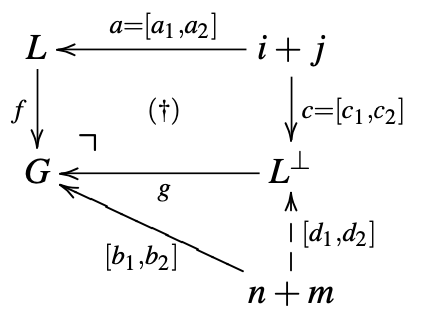
\includegraphics[width=0.4\linewidth]{figures/combinatorial_semantics/boundary_complement.png}
% \end{figure}
% https://q.uiver.app/#q=WzAsNSxbMCwwLCJMIl0sWzIsMCwiaStqIl0sWzAsMiwiR157XFx1cmNvcm5lcn0iXSxbMiw0LCJuK20iXSxbMiwyLCJMXntcXGJvdH0iXSxbMyw0LCJbZF8xLGRfMl0iLDJdLFszLDIsIltiXzEsYl8yXSJdLFswLDIsImYiLDJdLFsxLDAsImEgPSBbYV8xLGFfMl0iLDJdLFsxLDQsImMgPSBbY18xLGNfMl0iXSxbNCwyLCJnIl1d
% \[\begin{tikzcd}
% 	\mathcal L && {i+j} \\
% 	\\
% 	{\mathcal G^{\urcorner}} && {\mathcal{L}^{\bot}} \\
% 	\\
% 	&& {n+m}
% 	\arrow["{[d_1,d_2]}"', from=5-3, to=3-3]
% 	\arrow["{[b_1,b_2]}", from=5-3, to=3-1]
% 	\arrow["f"', from=1-1, to=3-1]
% 	\arrow["{[a_1,a_2]}"', from=1-3, to=1-1]
% 	\arrow["{[c_1,c_2]}", from=1-3, to=3-3]
% 	\arrow[from=3-3, to=3-1]
% \end{tikzcd}\]
\[
    \scalebox{0.8}{
        \tikzfig{../figures/combinatorial_semantics/DPOI_boundary_complement}
    }
\]
is called a boundary complement if $[c_1, c_2]$ is mono and there exist $d_1 : n \to \mathcal{L}^{\bot}$ and $d_2 : m \to \mathcal{L}^{\bot}$ making the above triangle commute and such that
\[
    n + j \xrightarrow{[d_1,c_2]} \mathcal{L}^{\bot} \xleftarrow{[d_2,c_1]} m + i
\]
is an MDA cospan. 
\end{definition}

Intuitively,  requiring boundary complements ensures that inputs are glued exclusively to outputs and vice-versa in the two pushout squares.
Yet, this restriction is not enough to make DPOI rewriting complete for $\catname{S}(\Sigma,\mathcal{E})$: there might be cospans with carriers $\mathcal{G}$ and $\mathcal{H}$ such that one can be rewritten into another but their corresponding morphisms are not equal modulo $\mathcal{E}$~\cite{bonchi_string_2022-2}.
To make the DPOI rewriting complete, we need to add a restriction on the image of the match.

\begin{definition}[Convex match]
We call a subgraph $\mathcal{H}$ of a hypergraph $\mathcal{G}$ a \emph{convex subgraph} if for all $v_i, v_j \in V_{\mathcal{H}}$ every path from $v_i$ to $v_j$ is also in $\mathcal{H}$.
We call a match $f : \mathcal L \to \mathcal G$ a \emph{convex match} if it is mono and its image is a convex subgraph of $\mathcal G$. 
   
\end{definition}

\begin{definition}[Convex DPOI rewriting]
\label{def:convex_dpo}
Let $\mathfrak{R}$ be a set of DPOI rewrite rules. 
Then, given $\mathcal G \xleftarrow{} n+m$ and $\mathcal H \xleftarrow{} n + m$ in $\catname{Hyp(\Sigma)}$, $\mathcal G$ rewrites convexly into $\mathcal H$ with interface $n + m$ --- notation $(\mathcal G \xleftarrow{} n + m ) \Rrightarrow_{\mathfrak{R}}  (\mathcal H \xleftarrow{} n + m )$ --- if there exist rule $\mathcal L \xleftarrow{} i + j \xrightarrow{} \mathcal R$ in $\mathfrak{R}$ and object $\mathcal{L}^{\bot}$ and cospan arrows $i+j \xrightarrow{} \mathcal{L}^{\bot} \xleftarrow{} n+m$ such that the DPOI diagram of Definition \ref{def:dpoi} commutes and its marked squares are pushouts 
and the following conditions hold
\begin{itemize}
    \item $f : L \to \mathcal G$ is a convex match;
    \item $i + j \to \mathcal{L}^{\bot} \to \mathcal G$ is a boundary complement in the leftmost pushout.
\end{itemize}
\end{definition}

We do not formally recite the main result of \cite{bonchi_string_2022-2} here,  but the work proves that for any morphisms $f$ and $g$ in $\catname{S}(\Sigma, \mathcal{E})$,  we have that $f = g$ if and only if there exist a sequence of DPO rewrites (induced by $\mathcal{E}$) between the representations of $f$ and $g$ as (cospans of) hypergraphs.
In particular,  Theorem \ref{thm:prop-equiv} means that the structural SMC equations are factored out in the representation of $f$ and $g$,  and the DPO rewrites necessary are only those induced by $\mathcal{E}$. 

We extend the definition of e-hypergraphs for $\catname{SLat}$-enriched symmetric monoidal categories~\cite{ghica2024equivalencehypergraphsegraphsmonoidal} to accommodate new structure brought by closedness.


\begin{definition}
We define an e-hypergraph $\mathcal{G}$ over a closed symmetric monoidal signature $\Sigma = (\Sigma_{O}, \Sigma_{M})$ as a tuple $(V,E,s,t, l_{V}, l_{E} \textcolor{red}{<}, \textcolor{blue}{<},\consistency)$ where
\begin{itemize}
  \item $V$ is a set of vertices.
  \item $E = \colorbox{yellow}{E} \cup \textcolor{red}{E} \cup \textcolor{blue}{E}$ is a set of hyperedges that that is formed of three disjoint sets of hyperedges defined below.
  \item $s,t : E \to V^{*}$ are source and target functions.
  \item $l_{E} : E \to \Sigma_{M} + 1$, $l_{V} : V \to \Sigma_{O} \cup \text{obj}_{\multimap}$ are \textit{label} functions, where $\text{obj}_{\multimap}$ consists of objects $A \multimap B$ for $A,B \in obj_{\Sigma_{O}}$.
  \item $\textcolor{red}{<} \subseteq \textcolor{red}{E} \times V + E$ and $\textcolor{blue}{<} \subseteq \textcolor{blue}{E} \times V + E $ with $\textcolor{red}{E}, \textcolor{blue} \subset E$ are disjoint partial orders that are defined as a transitive closure of corresponding immediate predecessor relations that we denote as $\textcolor{red}{<^{\mu}}$ and $\textcolor{blue}{<^{\mu}}$.
        For $x \in V + E$, the set of predecessors of $x$ is denoted as $[x) = \{x' ~|~ \exists y_{1} = x', \ldots, y_{n} = x,  y_{i} \textcolor{red}{<^{\mu}} y_{i + 1} \text{ or } y_{i} \textcolor{blue}{<^{\mu}} y_{i+1}\; \}$.
        We call edges $e$ such that $l(e) = \bot$ hierarchical and edges $e$ and vertices $v$ such that $[e) = \varnothing$ and $[v) = \varnothing$ \textit{top-level}.
        Each of these relations should satisfy the following
        \begin{enumerate}
          \item each set of predecessors consists exclusively of hierarchical edges;
          \item each $x$ has at most one immediate predecessor;
          \item edges $e$ such that there is no $x$ such that $e \textcolor{red}{<^{\mu}} x$ or $e \textcolor{red}{<^{\mu}} x$ are labelled;
          \item the relations are closed under connectivity, \emph{i.e.}, if $v \in s(e)$ then $e' \textcolor{red}{<^{\mu}} e$ iff $e' \textcolor{red}{<^{\mu}} v$, similarly for $v \in t(e)$ and $\textcolor{blue}{<}$.
        \end{enumerate}
  \item $\consistency$ is a \textit{consistency relation} which is given by the union of a family of equivalence relations $\consistency_p$ on each set $\{x \in V + E ~|~ p \textcolor{red}{<^\mu} x\}$ of elements which share the same parent where each relation is also closed under connectivity, \textit{i.e.}, if $v \in s(e)$ or $v \in t(e)$ such that $p \textcolor{red}{<^{\mu}}(v)$ and $p \textcolor{red}{<^{\mu}}(e)$ then $v \consistency_{p} e$.
  We require that $\consistency_{p} \not = (E_{p} + V_{p}) \times (E_{p} + V_{p})$ where $V_{p} = \{ v ~ | ~ p \textcolor{red}{<^{\mu}} v\}$ and $E_{p} = \{ e ~ | ~ p \textcolor{red}{<^{\mu}} e\}$.
\end{itemize} 
$\textcolor{red}{E}$ and $\textcolor{blue}{E}$ are then induced by the corresponding relations can consist of exclusively hierarchical edges, then we have $\colorbox{yellow}{E} = E \setminus \textcolor{red}{E} \cup \textcolor{blue}{E}$.
Given an e-hypergraph $\mathcal{G}$ we can consider a corresponding \textit{underlying} hypergraph $\mathcal{G}'$ by forgetting $<$ and~$\consistency$.
\end{definition}

Intuitively, edges from $\textcolor{red}{E}$ encode equivalence classes, \emph{i.e.}, e-boxes, while edges from $\textcolor{blue}{E}$ encode lambda-abstraction boxes.
Also note the typing on the $l_{V}$ function.
We work with freely generated closed semilattice-enriched categories and to avoid unnecessary complications we limit the labelling of vertices to such a type.
In particular, it prohibits vertices to be labelled with, \emph{e.g.}, $A \otimes B$, but allows them to be labelled with $A \otimes B \multimap C \otimes D$.

Consider an example in the middle part of Figure~\ref{fig:e-cospan-example}.
The e-hypergraph in the example is given by $V = \{v_{1}, \ldots w_{10}\}$, $E = \{e_{1}, \ldots, e_{7}\}$, $\textcolor{red}{E} = \{e_{1}\}$, $\textcolor{blue}{E} = \{e_{2}\}$, $l_{E} = {e_{1} \mapsto \bot, e_{2} \mapsto \bot, e_{3} \mapsto g, \ldots, e_{7} \mapsto f}$ and then we have
\[
\begin{array}{cccc}
  v_{4} \textcolor{red}{<^{\mu}} e_{1} & v_{7} \textcolor{blue}{<^{\mu}} e_{2} & v_{4} \consistency e_{2} & v_{4} \not \consistency v_{10}\\
  e_{3} \textcolor{red}{<^{\mu}} e_{1} & v_{8} \textcolor{blue}{<^{\mu}} e_{2} &  e_{2} \consistency u_{1} & e_{2} \not \consistency e_{6}\\
  e_{2} \textcolor{red}{<^{\mu}} e_{1} & e_{5} \textcolor{blue}{<^{\mu}} e_{2} & e_{2} \consistency e_{4} & e_{4} \not \consistency e_{7}\\  
  \ldots & \ldots & \ldots & \ldots \\
  v_{12} \textcolor{red}{<^{\mu}} e_{1} & w_{9} \textcolor{blue}{<^{\mu}} e_{2} & v_{11} \consistency v_{12} & w_{6} \not \consistency w_{10}
\end{array}
\]
and, in particular, we have $[e_{5}) = \{e_2, e_1\}$.
$\consistency_{e_{1}}$ defines a partition on immediate successors of $e_{1}$ which we delimit by a vertical dashed line.
Edges in $\textcolor{red}{E}$ are depicted with a dashed box, while edges in $\textcolor{blue}{E}$ --- with a round solid box.

\begin{figure}

\[
\adjustbox{scale=0.6}{
\tikzfig{./figures/closed_iso_example_2}
}
\]
\caption{Cospan of e-hypergraphs example}
\label{fig:e-cospan-example}
\end{figure}

\begin{definition}[E-hypergraph homomorphism]
  An \textit{e-hypergraph homomorphism} $\phi:\mathcal{F}\to\mathcal{G}$ between e-hypergraphs $\mathcal{F},\mathcal{G}$ is a pair of functions $\phi_V : V_{\mathcal{F}} \to V_{\mathcal{G}}, \phi_E : E_{\mathcal{F}} \to E_{\mathcal{G}}$ such that
  \begin{enumerate}
      \item $\phi$ is a hypergraph homomorphism;
      \item $\phi_{E}(\textcolor{red}{E_{\mathcal{F}}}) \subseteq \textcolor{red}{E_{\mathcal{G}}}$ and $\phi_{E}(\textcolor{blue}{E_{\mathcal{F}}}) \subseteq \textcolor{blue}{E_{\mathcal{G}}}$;
      \item for $v \in V_{\mathcal{F}}$ and $e \in E_{\mathcal{F}}$
        \begin{align*}
          &\text{if } e \textcolor{red}{<_{\mathcal{F}}^{\mu}} v \text{ then } \phi(e) \textcolor{red}{<_{\mathcal{G}}^{\mu}} \phi(v)\\
          &\text{and}\\
          &\text{if } e \textcolor{blue}{<_{\mathcal{F}}^{\mu}} v \text{ then } \phi(e) \textcolor{blue}{<_{\mathcal{G}}^{\mu}} \phi(v)
        \end{align*}
          and for $e_1, e_2 \in E_{\mathcal{F}}$
          \begin{align*}
          &\text{if } e_1 \textcolor{red}{<_{\mathcal{F}}^{\mu}} e_2 \text{ then } \phi(e_1) \textcolor{red}{<_{\mathcal{G}}^{\mu}} \phi(e_2)\\
          &\text{and}\\
          &\text{if } e_1 \textcolor{blue}{<_{\mathcal{F}}^{\mu}} e_2 \text{ then } \phi(e_1) \textcolor{blue}{<_{\mathcal{G}}^{\mu}} \phi(e_2)
          \end{align*}
          \item for all $x_1, x_2 \in \mathcal{F}$,  $x_1 ~\consistency_{\mathcal{F}}~ x_2$ implies $\phi(x_1) ~\consistency_{\mathcal{G}}~ \phi(x_2)$. 
  \end{enumerate}
  % If we further have that if $[x_1) = \varnothing$ then $[\phi(x_1)) = \varnothing$ we call the homomorphism \textit{strict}.
  \end{definition}
  The conditions on e-hypergraph homomorphisms require preserving immediate predecessors and the consistency relation.
  \begin{definition}[Category of e-hypergraphs]
  The \emph{category of e-hypergraphs},  denoted  $\catname{EHyp(\Sigma)}$,  has e-hypergraphs as objects and e-hypergraph homomorphisms as morphisms.  
  \end{definition}

The category of e-hypergraphs has coproducts,  given by the disjoint union of e-hypergraphs,  and an initial object given by the empty e-hypergraph.  
A concrete description of the pushout of two morphisms in this category is given in the Appendix section~\ref{sec:appendix:pushout}.
Generally,  the pushout of two e-hypergraph homomorphisms need not exist,  but it does when certain technical conditions are satisfied. 
Most importantly a pushout for the composition of two cospans with discrete feet exists, as described below.
  
As in the case of $\catname{S}(\Sigma)$ and $\MdaCospans$, e-hypergraphs requires interfaces in order to model string diagrams with dedicated inputs and outputs.
Because string diagrams for closed semilattice-enriched symmetric monoidal categories are nested, containing substring diagrams inside e-boxes and lambda abstraction boxes, we need to account for the interfaces in these nested contexts as well.
Nested inputs and outputs of a string diagram do not participate in composition of string diagrams, hence they need to be distinguished from the ones that participate in the composition.
We thus propose \textit{extended} cospans of discrete e-hypergraphs and use the notation $n \setminus m$ to denote the discrete e-hypergraph with $n \setminus m$ vertices, in particular
with the vertices of $m$ removed from $n$ when vertices of $m$ is a sub-e-hypergraph of $n$.

\begin{definition}[Category of e-hypergraphs with interfaces]
  The category of \textit{e-hypergraphs with extended interfaces} $\Ecospans$ has discrete \textit{ordered} e-hypergraphs as objects,  with hom-sets $\Ecospans(n,m)$ consisting of isomorphism classes (defined below) of \textit{extended cospans}, defined as follows:  
  \[
  n \xrightarrow{f_{ext}} n' \xrightarrow{f_{int}} \mathcal{G} \xleftarrow{g_{int}} m' \xleftarrow{g_{ext}} m
  \]
  where $\mathcal{G}$ is an e-hypergraph,  and $n, n', m, m'$ are discrete ordered e-hypergraphs,  $f_{ext},g_{ext}$ are monomorphisms in $\catname{EHyp(\Sigma)}$,  and the image of $f_{ext};f_{int}$ and of $g_{ext};g_{int}$ consist exclusively of top-level vertices,  and such that vertices in the strictly internal interface (defined below) are not top-level.  
  We sometimes write $\mathcal G$ to denote the extended cospan,  where it is clear from context $\mathcal G$ is equipped with extended interfaces. 

\end{definition}
We call $n$  \textit{external input interfaces}, $n'$ \textit{internal input interfaces},
and $n' \setminus f_{ext}(n)$  the \textit{strictly internal input interfaces}.  
We do analogously for the \emph{output interfaces},  with respect to $m$,  $m'$ and $m' \setminus g_{ext}(m)$.  
We occasionally conflate $f_{ext}$ with $f_{ext};f_{int}$ when it is clear from context,  and also conflate $n$ and $m$ with their images in $n'$ and $m'$,  and likewise $m, m, n', m'$ with their images in $\mathcal{G}$. 
Given an edge $e \in E_\mathcal{G}$ such that $l(e) = \bot$,  we call the \textit{inputs of $e$} the intersection of the strictly internal input interface of $\mathcal{G}$ with the immediate successors of $e$,  and analogously for the \emph{outputs of $e$}.
Graphically, we depict such extended cospans as in Figure~\ref{fig:e-cospan-example}: feet of the cospan are depicted within shaded regions.
All non-black vertices form strictly internal interfaces.


\begin{definition}[Isomorphic cospans]
Consider a relation 
\begin{multline*}
R = \{ x R y \text{ if } f_{\text{int}}(x) \consistency f_{\text{int}}(y)\\ \;\text{or}\; \exists z \;\text{s.t.}\; z \textcolor{blue}{<^{\mu}} f_{\text{int}}(x) \text{ and } z \textcolor{blue}{<}^{\mu} f_{\text{int}}(y)\}
\end{multline*}
for $x, y \in n'$.
And let $S$ be its reflexive closure.
The latter partitions $n'$ into non-empty subsets $\{p_{j}\}^{k}_{j=1}$.
We get an analogous partition for $m'$.

Two extended cospans are isomorphic if there exist isomorphisms $\alpha$, $\beta$ and $\gamma$ making the following diagram commute and such that $\alpha$ and $\gamma$ preserve order within each $p_j$.
\[
\scalebox{0.8}{
    \tikzfig{../../figures/combinatorial_semantics/isomorphic_e_cospans}
}
\]
\end{definition}

In Figure~\ref{fig:e-cospan-example} the partitions for input and output internal interfaces are given with colours.

Composition of two morphisms 
\begin{align*}
	n \xrightarrow{f_{ext}} n' \xrightarrow{f_{int}} &\mathcal{F} \xleftarrow{f'_{int}} m' \xleftarrow{f'_{ext}} m\\
	m \xrightarrow{g_{ext}} m'\!' \xrightarrow{g_{int}} &\mathcal{G} \xleftarrow{g'_{int}} k' \xleftarrow{g'_{ext}} k
\end{align*} is computed in two stages.
First, $\mathcal{H}$ is computed as the result of the pushout square shown below; 
% https://q.uiver.app/#q=WzAsMTAsWzAsMCwiZXh0KFgpIl0sWzEsMSwiWCJdLFsyLDIsIkEiXSxbMywwLCJZIl0sWzQsMCwiZXh0KFkpIl0sWzUsMCwiWSciXSxbNiwyLCJCIl0sWzcsMSwiWiJdLFs4LDAsImV4dChaKSJdLFs0LDMsIl57XFx1bGNvcm5lcn1BK197Zl97ZXh0fTtmLGdfe2V4dH07Z31CIl0sWzAsMV0sWzEsMl0sWzMsMiwiZiJdLFs0LDMsImZfe2V4dH0iXSxbNCw1LCJnX3tleHR9IiwyXSxbNSw2LCJnIiwyXSxbNyw2XSxbOCw3XSxbMiw5XSxbNiw5XV0=
\[
\trimbox{0cm 0cm 0cm 0.75cm}{
\adjustbox{scale=0.9,center}
{\tikzfig{./figures/pushout_e_cospans}}
}
\]
then,  the result of composition is defined as follows:
\[
n \xrightarrow{f_{ext};\iota_1} n' + (m'' \setminus m) \xrightarrow{h_{1}} \mathcal{H} \xleftarrow{h_2} k' + (m' \setminus m) \xleftarrow{g'_{ext};\iota_1} k
\]
where $h_i$ are defined as follows,  using $|$ to denote the restriction of a function on a discrete e-hypergraph. 
\begin{align*}
    h_1 = [ f_{int};p_1, ~(g_{int};p_2)|_{m'' \setminus m} ]
\\
    h_2 = [ g'_{int};p_2, ~(f'_{int};p_1)|_{m' \setminus m} ]
\end{align*}
% \[
% \begin{tikzcd}
% Y_{ext} \arrow[d] & 0 \arrow[l] \arrow[d]    \\
% Y'          & Y' \setminus Y_{ext} \arrow[l]
% \end{tikzcd}
% \]
% and then the disjoint union is just a coproduct. 
% where $g'$ is the restriction of $g$ to ${Y' \setminus Y_{ext}}$ and $f'$ the restriction of $f$ to $Y \setminus Y_{ext}$. 
The identity of composition is given by the obvious extended cospan of identities. 
$\Ecospans$ inherits a symmetric monoidal structure from the coproduct (and initial object) structure of $\catname{EHyp({\Sigma}})$,  analogously to Definition~\ref{def:cspd}.
As in the standard cospan construction,  it is necessary to consider isomorphism classes of cospans since composition (defined by pushout) is associative only up-to isomorphism (since pushouts are unique only up-to isomorphism). 


For the same reasons as in the case of $\catname{S}(\Sigma)$ we restrict cospans to MDA cospans.
We also need to enforce typing constraints on hierarchical edges so that they represent well-typed closed $\Sigma^{+}$-terms.
\begin{definition}
  We call a cospan 
  \[
n \xrightarrow{f_{\text{ext}}} n' \xrightarrow{f_{\text{int}}} \mathcal{G} \xleftarrow{g'_{\text{int}}} m' \xleftarrow{g_{\text{ext}}} m
\]
monogamous directed acyclic if
\begin{itemize}
  \item underlying hypergraph of $\mathcal{G}$ is directed acyclic;
  \item in- and out- degrees of every vertex is at most 1;
  \item $f_{\text{int}}$ and $g_{\text{int}}$ are monos;
  \item vertices with in-degree (respectively, out-degree) of 0 are precisely the image of $f_{\text{int}}$ (respectively, $g_{\text{int}}$).
\end{itemize}

MDA cospans and discrete e-hypergraphs form a category $\MdaEcospans$.
\end{definition}

    
\begin{definition}
  We call a monogamous cospan
  \[
    n \xrightarrow{f_{\text{ext}}} n' \xrightarrow{f_{\text{int}}} \mathcal{G} \xleftarrow{g'_{\text{int}}} m' \xleftarrow{g_{\text{ext}}} m
  \]
  \textit{well-typed} if all hierarchical edges of $\mathcal{G}$ are well-typed in the sense below.
  \begin{itemize}
    \item For each $e \in \textcolor{red}{E}$ consider sets $I$ and $O$ of its input and output vertices partitioned according to $\consistency_{e}$.
          $e$ is well-typed if for each element $S$ of the partition of $I$ $w(S) = w(s(e))$ and similarly for $O$ and $t(e)$.
    \item For each $e \in \textcolor{blue}{E}$ consider sets $I$ and $O$ of its input and output vertices.
          $e$ is well-typed if there exists an object $B \in \text{obj}_{\Sigma_{O}}$ such that $[w(s(e)), B] = w(I)$ and $B \multimap w(O) = w(t(e))$.
  \end{itemize}

  We denote the category of well typed MDA cospans as $\WellTypedMdaEcospans$.
  \end{definition}
This is a proper category as identities, symmetries, and tensor unit are well-typed and composition and tensor product of two well-typed MDA cospans is again a well typed MDA cospan.

Consider, again, Figure ~\ref{fig:e-cospan-example}.
To make edge $e_{1}$ well-typed, it is necessary that $w([v_{4},v_{5},v_{6}]) = w([v_{10},v_{11},v_{12}]) = w([v_1,v_2,v_3])$ and $w([w_{4},w_{5},w_{6}]) = w([w_{10},v_{12},v_{11}]) = w([w_1,w_2,w_3])$ (note the change of ordering in the output of $e_{1}$).
To make edge $e_{2}$ well-typed, it is necessary that $w([v_4,v_5,v_9]) = w([v_7,v_8,v_9])$ and $w([u_1]) = w([v_9]) \multimap w([v_8,v_7,w_9])$.


Unlike in the previous section,  in order to give an equivalence with $\catname{S}^+(\Sigma)$,  we must first develop the theory of DPOI rewriting for e-hypergraphs.
This is because the equations for semilattice enrichment are not intended to be subsumed by the e-hypergraph representation, apart from the commutativity equation which is absorbed by the definition of isomorphic cospans.
Instead,  we treat them via rewriting,  as we do with equations of the signaturem because the semilattice equations involve sharing and copying, operations on string diagrams which are not usually quotiented away.
% , cf. string diagrams for Cartesian categories.  
An ideal combinatorial representation would factor out the two semilattice equations which \textit{do not} involve sharing and copying (namely,  associativity and idempotence) --- however, a limitation of the current work is that we do not achieve this,  so we also handle these equations via rewriting. 

\section{DPOI-Rewriting for E-Hypergraphs}

Because extended cospans have a more general notion of interface,  including \textit{internal} vertices,  DPOI rewriting as presented in Section \ref{sec:combinatorial-semantics} needs some adjustments, defined in this section. 

We do not expect internal interfaces to be preserved during rewriting: for example,  when the semilattice equations are considered as rewrites. 
Thus,  we wish a rewrite rule to be a pair of \textit{extended} cospans of e-hypergraphs with matching \textit{external} (but not necessarily internal) interfaces,  as follows. 
\[
    n \xrightarrow{} n' \xrightarrow{} \mathcal{L} \xleftarrow{} m' \xleftarrow{} m
\qquad
    n \xrightarrow{} n'' \xrightarrow{} \mathcal{R} \xleftarrow{} m'' \xleftarrow{} m
\] 
Analogous to Section \ref{sec:combinatorial-semantics}, observing that the following extended cospans express the same data
\[
    0 \xrightarrow{} 0 \xrightarrow{} \mathcal{L} \xleftarrow{} n'' + m'' \xleftarrow{} n + m
\qquad
    0 \xrightarrow{} 0 \xrightarrow{} \mathcal{R} \xleftarrow{} n' + m' \xleftarrow{} n + m
\] allows us to encode rewrite rules as extended cospans of the following form
\[
\mathcal{L} \xleftarrow{} n' + m' \xleftarrow{} n + m \xrightarrow{} n'' + m'' \xrightarrow{} \mathcal{R}
\] 
which fits into the DPO formalism. We make this identification throughout,  without further mention. 
%We will futher omit the arrows $0 \to 0 \to \mathcal{L}$.
\begin{remark}
The extended DPOI rewriting as defined in this section trades off simplicity for expressiveness: it is unable to express rewriting for rules whose source or target contain a maximal connected sub-hypergraph with no input and output vertices.
While this limitation can be overcome by specifically encoding such rewrite rules, we find the technical development to be simpler if we avoid consideration of such rules and therefore consider signatures which can not result in construction of terms with type $0 \to 0$. 
This limitation has no practical impact in applications of interest. 
However, the general case without this limitation can be found in Section~\ref{sec:dpo-fix} of the Appendix.
%This is because there is no way to impose both consistency and child relation of such an edge as it has no incident nodes in its context.
%We claim that this is only a minor limitation because in practice such edges (morphisms) with no
%incident nodes correspond to ‘scalars’, if we consider for example a category of vector spaces, and scalars are usually removed by being absorbed by vectors rather than introduced during rewrites.
\end{remark}


% The input interface on the left-hand side of the rule is $\{1, 2\}$, while the input interface on the right-hand side of the rule is $\{1,2,5,6,7,8\}$.
% Note that the outermost interfaces are preserved.

% Another concern is when we delete the occurrence of the left-hand side of a rewrite rule from an e-hypergraph we also modify this e-hypergraph's interfaces.
% Consider a hypothetical DPO square below in Figure~\ref{fig:interface_change_example} where long arrows denote matching between carriers of cospans.

% The first row of the diagram shows the span for a rewrite rule of $\langle f + g, f \rangle$ which is like a projection rule.
% Note once again the difference between the interfaces of the left-hand and right-hand sides of the rewrite rule.
% The entry in the middle of the span depicts the outermost interfaces which are preserved.
% The second row depicts the e-hypergraph to be rewritten on the left and the result of the rewrite on the right.
% The result is obtained by first deleting the image of the left-hand side of the rewrite rule from the initial e-hypergraph (depicted in the middle) and then gluing the right-hand side of the rewrite rule into it. 
% Note that the interfaces of the initial e-hypergraph and the residual e-hypergraph are different. 
% Here, the outermost and the whole interfaces for the eventual e-hypergraph coincide, but if the nested-ness of the initial e-hypergraph was more intense the result could have inner interfaces as well as we would remove the interfaces of the inner edges when deleting the image of the left-hand side part of the rule from the initial e-hypergraph.


Before introducing \textit{extended} DPOI rewriting,  the definition of boundary complement must guarantee that rewriting yields a monogamous directed acyclic e-hypergraph. 
First,  we introduce the  ancillary notion of a \textit{down-closed} graph:
\begin{definition}[Down-closed subgraph]
%A \textit{subgraph} of $\mathcal G $ an e-hypergraph $\mathcal H$ 
%is an e-hypergraph whose edge and vertex sets are subsets of those of $\mathcal H$, 
%and whose remaining equipment is a restriction of that of $\mathcal H$ to those sets. 
    We call  a sub-e-hypergraph $\mathcal G $ of $\mathcal H$ \emph{down-closed} if for all $e \in E_{\mathcal{G}}$,   all children of $e$ are also in $\mathcal{G}$.
\end{definition}    

\begin{definition}[Extended boundary complement]
\label{def:boundary_new}

% https://q.uiver.app/#q=WzAsNyxbMiwwLCJMIl0sWzQsMCwieF97ZXh0fSArIHlfe2V4dH0iXSxbMiwyLCJHXntcXHVyY29ybmVyfSJdLFs0LDIsIkMiXSxbNCw0LCJuX3tleHR9K21fe2V4dH0iXSxbMCwwLCJsX2krbF9vIl0sWzAsMiwiZ19pK2dfbyJdLFsxLDAsIiIsMCx7ImNvbG91ciI6WzAsNjAsNjBdfV0sWzAsMiwibSIsMCx7ImNvbG91ciI6WzAsNjAsNjBdfSxbMCw2MCw2MCwxXV0sWzEsMywiW2lfYyxqX2NdIiwwLHsiY29sb3VyIjpbMCw2MCw2MF19LFswLDYwLDYwLDFdXSxbNCwzLCJbbl9jLG1fY10iLDIseyJjb2xvdXIiOlswLDYwLDYwXX0sWzAsNjAsNjAsMV1dLFszLDIsIiIsMix7ImNvbG91ciI6WzAsNjAsNjBdfV0sWzQsMiwiIiwyLHsiY29sb3VyIjpbMCw2MCw2MF19XSxbNSwwXSxbNiwyXV0=

For MDA cospans 
\[
    i \xrightarrow{} i' \xrightarrow{} \mathcal{L} \xleftarrow{} j' \xleftarrow{} j
\quad\text{ and }\quad
    n \xrightarrow{} n' \xrightarrow{} \mathcal{G} \xleftarrow{} k' \xleftarrow{} k
\] and mono $m : \mathcal{L} \to \mathcal{G}$ in $\catname{EHyp(\Sigma)}$, a pushout complement $i + j \to \mathcal{L}^{\bot} \to \mathcal{G}$
as depicted in the square below
\[
\scalebox{0.75}{

    \tikzfig{./figures/DPOI_pushout_complement}
}
\]
is a \textit{boundary complement} if
\begin{enumerate} 
    \item $m(\mathcal L)$ is a convex down-closed e-hypergraph;
    \item $[c_1,c_2]$ is mono;
    \item for all $v,w$ in $\mathcal{G}$ in the image of $i + j$,  $v$ and $w$ share the same set of parents, and either $v,w$ are top-level or else $v \consistency w$;
    \item for all $v,w$ in $\mathcal{L}^{\bot}$ in the image of $i + j$,  $v$ and $w$ share the same set of parents, and either $v,w$ are top-level or else $v \consistency w$;
    \item there exist $d_1 : n \to \mathcal{L}^\bot$ and $d_2 : k \to \mathcal{L}^\bot$ making the above triangle commute; and
    \item if the image of $\mathcal{L}$'s external interfaces under $m$ consists exclusively of top-level vertices of $\mathcal{G}$ then there exists a \textit{well-typed} extended MDA cospan
    \[
    n + j \xrightarrow{f_1 + id_{j}} n' \setminus (i' \setminus i) + j \xrightarrow{[g_1,c_2]} \mathcal{L}^{\bot} \xleftarrow{[g_2,c_1]} k' \setminus (j' \setminus j) + i \xleftarrow{f_2 + id_{i}} k + i
    \]
    \item if the image of $\mathcal{L}$'s external interfaces under $m$ consists exclusively of not top-level vertices of $\mathcal{G}$ then there exists a \textit{not necessarily well-typed} extended MDA cospan
    \[
    n \xrightarrow{f_1} n' \setminus (i' \setminus i) + j \xrightarrow{[g_1,c_2]} \mathcal{L}^{\bot} \xleftarrow{[g_2,c_1]} k' \setminus (j' \setminus j) + i \xleftarrow{f_2} k
    \]
\end{enumerate}
where $f_i$ and $g_i$ are defined as follows.  
 %because the image of $m$ is a convex down-closed e-hypergraph, 
The strictly internal interface $i' \setminus i$ of $\mathcal L$ is mapped to the internal interface $n'$ of $\mathcal G$,  since $\mathcal L$ is a down-closed subgraph of $\mathcal G$,  inducing an identification of $i' \setminus i$ in  $n'$. 
Then map $f_1$ is given by $g_{ext}$ with its codomain restricted to $n' \setminus (i' \setminus i)$.\footnote{Noting the image of $g_{ext}$ indeed lies within $n' \setminus (i' \setminus i)$}  The map $g_1$ is derived from the restriction of $g_{int}$ to type $n' \setminus (i' \setminus i) \to \mathcal G$ by further observing that $\mathcal L^\bot$ can be identified within $\mathcal G$ --- and in particular has the internal interface $n'$ of $\mathcal G$ minus $i' \setminus i$.  The maps $f_2$ and $g_2$ are defined similarly. 
%$i' \setminus i$, which is a strict internal interface of $\mathcal{L}$, is necessarily mapped to vertices in the strict internal interface of $\mathcal{G}$ which are also in the image of $n'$ and therefore we can construct a 
%morphism $f' : i' \setminus i \to n'$ by first following $m$ and then composing with the partial inverse of $g_{int}$ which exists because it is mono. 
%Then we define $n' \setminus (i' \setminus i)$ as the pushout complement in the diagram below
%
%\[
%    \tikzfig{combinatorial_semantics/pushout_difference}
%\]
%and $g_1$ is obtained by composition $g';g_{int}$ and then composing with the inverse of $l$.
%Similarly for $g_2$.
% CHRIS: TRY TO DEFINE G1, G2 AS SIMPLY AS POSSIBLE, AND POSSIBLY ADD AN INFORMAL EXPLANATION BELOW THE DEFINITION. 
% Because $\mathcal{L}^{\bot}$ is essentially $\mathcal{G}$ with $\mathcal{L}$ removed, apart from the part that has a pre-image in $i + j$, there is an obvious morphism from $l \to \mathcal{L}^{\bot}$ which is $g_1 = g_{int} |_{D}$ where
% \[
%     D = \{ v \in n' \text{ such that } \not \exists u \in (i' \setminus i) ~ . ~ g_{int}(v) = f'_{int};f(u) \}
% \]
% Similarly for $r \to \mathcal{L}^{\bot}$, which we denote as $g_2$.
% Then there exists a morphism $n \to l$, because there is a morphism $n \to n'$ and the external interfaces of $n'$ and $l$ are the same.
% That is, it is a morphism $f: n \to l$ such that $d_1 = f;g_1$.
% Similarly for $k \to r$.
\end{definition}

Intuitively speaking, the above definition means that when the occurrence of $\mathcal{L}$ within $\mathcal{G}$ is top-level then $\mathcal{L}$'s external interfaces become the part of $\mathcal{L}^{\bot}$'s external interfaces and when the occurrence is nested, those interfaces become the part of $\mathcal{L}^{\bot}$'s strict internal interfaces.
In both cases when removing the occurrence of $\mathcal{L}$ from $\mathcal{G}$, $\mathcal{L}$'s strict internal interfaces are removed from strict internal interfaces of $\mathcal{G}$ to form internal interfaces of the corresponding MDA cospans above.
The morphisms are then constructed correspondingly to require that inputs (respectively, outputs) of $\mathcal{R}$ are glued to the outputs (respectively, inputs) of $\mathcal{L}^{\bot}$.

%The notion of a boundary complement above is essentially the same as the one from Section~\ref{sec:combinatorial-semantics}.
%CHRIS: THE FOLLOWING SENTENCE IS UNCLEAR. 
%The only difference is that we account for internal interfaces to require monogamous-ness and these interfaces must be computed explicitly to define the monogamous cospan.
%
%\begin{figure}
%    \centering
%    \[
%    \scalebox{0.5}{\tikzfig{combinatorial_semantics/interfaces_change_example}}\]
%    \caption{Hypothetical DPO square for $\catname{MACsp_{D}(EHyp_{\Sigma})}$}
%    \label{fig:interface_change_example}
%\end{figure}

% The second point above means that when cutting the mono-occurrence of $L$ out from $G$ we also need to remove the inner interfaces of $L$ from the whole interface of $G$. \question{According to the pushout squares above, $c_i$ is constructed by removing from $g_i$ everything from $l_i$ which does not have a pre-image in $i$, i.e., everything except the outermost interfaces (same holds for $c_o$)}

Note that,  in the above definition,  the extended cospan 
    \[
    n \xrightarrow{} n' \setminus (i' \setminus i) + j \xrightarrow{[g_1,c_2]} \mathcal{L}^{\bot} \xleftarrow{[g_2,c_1]} k' \setminus (j' \setminus j) + i \xleftarrow{} k
    \]
 is not necessarily well-typed.
This is because its input internal interface may contain vertices that previously were a part of the output internal interface and vice versa.
\begin{remark}
The boundary complement conditions, in particular, prohibit finding a match for $\mathcal L$ in $\mathcal G$,  below.  
\[
	\mathcal{L} = \scalebox{0.8}{\tikzfig{./figures/f_times_g}} \qquad \mathcal{G} = \scalebox{0.6}{\tikzfig{./figures/f_plus_g_inline}}
\]
\end{remark}

\begin{proposition}
\label{prop:boundary_unique}
    The boundary complement in~\ref{def:boundary_new} when exists is unique.
\end{proposition}

We are now ready to define \textit{convex extended DPOI (EDPOI) rewriting} for $\catname{EHyp({\Sigma})}$.  
It is analogous to Definition~\ref{def:convex_dpo},  except we must construct internal interfaces explicitly.
More precisely, when removing the occurrence of $\mathcal{L}$ from $\mathcal{G}$, \emph{i.e.}, by computing the pushout complement, the internal interfaces of the resulting e-hypergraph should be modified to \textit{exclude} the vertices corresponding to $\mathcal{L}$'s strictly internal interfaces (since the vertices they map to have been removed). 
Then, when gluing $\mathcal{R}$ into the hole,  the internal interfaces of the resulting e-hypergraph should be modified to \textit{include} the strictly internal interfaces of $\mathcal{R}$ (since new internal interfaces for them to map to have been added).

\begin{definition}[Convex EDPOI rewriting]
\label{def:dpoi-e}
Given an extended span of morphisms 
\[
    \mathcal{G} \xleftarrow{} n' + k' \xleftarrow{} n + k \xrightarrow{} n'' + k'' \xrightarrow{} \mathcal{H}
\]
in $\catname{EHyp(\Sigma)}$, we say $\mathcal{G}$ \textit{rewrites (convexly) to} $\mathcal{H}$ (\textit{with external interface} $n + k$ and \textit{taking internal interface} $n'+k'$ \textit{to} $n'' + k''$) --- denoted by $\mathcal{G} \Rrightarrow \mathcal H$  --- \textit{via a rewrite rule} 
\[
    \mathcal{L} \xleftarrow{} i' + j' \xleftarrow{} i + j \xrightarrow{} i'' + j'' \xrightarrow{} \mathcal{R}
\] 
if there exists an object $\mathcal{C}$ and morphisms which complete the following commutative diagram 
\[
 \scalebox{0.75}{
    \tikzfig{./figures/DPOI_square}
 }
\]
such that the two marked squares are pushouts and the following conditions hold:
    \begin{enumerate}
        \label{dpoi-e:assumptions}
       % \item $m : \mathcal{L} \to \mathcal{G}$ is a convex match;
        %\item $m(L)$ is a down-closed e-hypergraph;
        \item $i + j \to \mathcal{C} \to \mathcal{G}$ is a boundary complement;
	\item the internal interfaces of $\mathcal H$ are such that:
	\[
		n'' = n' \setminus (i' \setminus i) + (i'' \setminus i) \qquad k'' = k' \setminus (j' \setminus j) +  (j'' \setminus j)\\
	\]
	\item the map $f_1 = [g_1,h_1]: n'' \to \mathcal H$ in the diagram above consists of $g_1$ as defined in Definition \ref{def:boundary_new} of boundary complement,  and $h_1$ which is the restriction of the composite $i'' \to \mathcal R \to \mathcal H$ to $i'' \setminus i$,  and similarly for the map $f_2: k'' \to \mathcal H$.  
    \end{enumerate}
% The internal interfaces of the resulting e-hypergraph $\mathcal{H}$ from the cospan
%  \[
%     \mathcal{H} \xleftarrow{} n'' + k'' \xleftarrow{} n + k
% \]
    Given  a set $\mathfrak{R}$ of EDPOI rewrite rules and e-hypergraphs with extended interfaces $\mathcal G$ and $\mathcal H$,  we write $\mathcal G \Rrightarrow_\mathfrak{R} \mathcal H$ if there exists a EDPOI rewrite in $\mathfrak R$ such that via it $\mathcal G$ rewrites to $\mathcal H$,  and we write $\mathcal G \Rrightarrow^*_\mathfrak{R} \mathcal H$ if there exists a sequence of such rewrites. 
\end{definition}
% Together, the conditions ensure the result of a rewrite is a well-typed MDA e-hypergraph. 

The enhanced definition of extended DPOI ensures that the combinatorial representation of semilattice-enriched SMCs is sound and complete, in an appropriate sense. 
